%!TEX root = ../main.tex
\section*{Plan détaillé}

Cette thèse peut s'approcher de deux manières différentes. En version longue, elle traite de la possibilité d'appliquer des modèles d'apprentissage par renforcement pour améliorer les séquences d'exercices données à un élève sur une plateforme en ligne. En version courte, elle peut se lire comme une thèse apportant des contributions fondamentales à des problèmes de bandits à plusieurs bras non-stationnaires. Commençons par présenter la version longue.

Cette thèse s'est déroulée dans le cadre du dispositif CIFRE avec l'entreprise Lelivrescolaire.fr. Cette entreprise a développé Afterclasse, un site de révision en ligne gratuitement accessible et massivement utilisé. Dans le Chapitre~\ref{ch:afterclasse}, on donne quelques éléments de contexte concernant Afterclasse et Lelivrescolaire.fr. Le but de la thèse y est précisé : améliorer la séquence d'exercices en fonction des résultats de chaque élève, avec un focus sur le court terme. En effet, les élèves "bachotent" sur la plateforme et sont assez peu engagés dans le temps. Il est donc naturel de chercher à les aider sur le court terme. Pour cela, il nous faut évaluer rapidement ce qu'ils savent et ce qu'ils ne savent pas et utiliser cette connaissance pour les réorienter vers les exercices qui leurs seraient les plus utiles.

Le Chapitre~\ref{ch:exploration} présente les modèles les plus classiques d'exploration-exploitation en machine learning. Cette revue de littérature peu mathématisée (par rapport au standard du domaine) a pour but de présenter de manière détaillée mais abordable les questions et les réponses apportées par la communauté du machine learning sur ce dilemme naturel entre exploration et exploitation. Une emphase particulière est mise sur les problèmes de bandits à plusieurs bras. Dans ces problèmes, un agent choisit séquentiellement parmi plusieurs actions et obtient une récompense dépendant de l'action choisit. Le but est de réussir à repérer les actions qui mènent aux plus fortes récompenses. Pour cela, le joueur doit accepter d'explorer - et donc de se tromper - les différentes options afin d'améliorer sa connaissance du problème. 

Plusieurs modèles de récompenses sont détaillés. Dans le modèle stochastique stationnaire (Section~\ref{sec:stoch-bandits}), chaque bras est lié à une distribution aléatoire. Le but est donc d'évaluer la moyenne de la distribution tout en quantifiant l'information manquante. Dans le modèle adversarial (Section~\ref{sec:adv-bandits}), la récompense est choisie par un adversaire et on cherche donc à repérer les actions les plus prolifiques tout en étant suffisamment imprédictible par l'adversaire. Dans les modèles stochastiques non-stationnaires (Section~\ref{sec:non-stationary}), la distribution associée à chaque bras peut changer au cours du temps ou en fonction des actions choisies. Cela mène à un double problème : d'estimation statistique d'une part (Quelle est la valeur courante ?), et de stratégie d'autre part (Comment puis-je me prémunir contre la non-stationarité ?). Enfin, les bandits contextuels (Section~\ref{sec:contextual}) lient les différentes actions à l'aide d'éléments de contexte. Ces éléments permettent d'envisager un très grand nombre d'actions qui ne seront pas toutes explorées : l'information sur les unes permettant d'extrapoler la valeur des autres. 

Finalement, on présente en Section~\ref{sec:rl} quelques fondamentaux d'apprentissage par renforcement (\emph{reinforcement learning}). Ce modèle est beaucoup plus général que les modèles de bandits car le joueur possède un état qu'il doit contrôler pour rester dans des zones à fortes récompenses. Ce modèle est très riche et permet d'apprendre des taches très complexes. Pour autant, il est très consommateur de données et ses meilleures réussites ont souvent lieu dans des dispositifs ou des données peuvent être simulées facilement.

Le Chapitre~\ref{ch:its} est consacré aux possibilités d'adaptation du modèle de bandits pour un usage éducatif. Lorsqu'on donne une question à un élève, on observe la réponse à cette question, ce qui est très similaire au \emph{feedback} du modèle de bandit. Cependant, nous notons quatre écueils fondamentaux (Section~\ref{sec:shortcomings}) qui entravent un tel usage. Tout d'abord, il est difficile d'associer la réponse d'un élève à une récompense pour l'algorithme. Faut-il privilégier les questions que l'élève réussit ou celles qu'il ne connaît pas ? Une fois la récompense posée, l'algorithme va tenter de la maximiser "brutalement": il faut donc faire très attention au proxy utilisé.




Deuxièmement, les modèles de bandits comparent souvent la performance obtenue à la performance de la "meilleure" action (inconnue). Dans le cas d'une séquence d'exercices, il est assez naturel qu'un exercice puissent être très intéressant à un instant donné, et beaucoup moins intéressant à l'avenir (par exemple, une fois que l'élève le maîtrise parfaitement). Il est donc essentiel de pouvoir se doter de points de comparaison plus intelligents que celui des bandits stationnaires ou adversariaux. 

Troisièmement, le modèle stationnaire suppose que ce qu'on observe ne réagit pas à nos actions. Dans le cas d'un système d'apprentissage, on souhaite que nos actions améliorent les performances de l'élève et que \emph{in fine} cela change les réponses qu'il envoie. Autrement dit, on souhaiterait pouvoir incorporer une modélisation de l'interaction entre l'élève et la machine.

Quatrièmement, les élèves font quelques dizaines de questions dans une séquence. C'est très peu, y compris pour un problème simple comme le problème des bandits stationnaires. Cet écueil s'oppose aux trois autres : là où ces derniers suggéraient une modélisation ambitieuse; ici, on doit se contenter de problèmes très simples.

À la Section~\ref{sec:bandits4ITS}, on détaille l'état de l'art de l'usage des modèles de bandits dans les systèmes d'apprentissage intelligents. Ces études empiriques très poussées s'attaquent à plusieurs objectifs, et montrent le plus souvent les comportements intéressants des algorithmes de bandits dans ces systèmes. Cependant, aucun de ces travaux ne s'attaque directement aux problèmes fondamentaux évoqués précédemment.

Dans le Chapitre~\ref{ch:rested}, on étudie la possibilité de faire travailler un élève sur le sujet le moins connu alors que celui-ci progresse au cours de ses révisions. Ainsi, on associe une récompense positive lorsque l'algorithme trouve une question qui n'est pas connue par l'élève (écueil 1). Au fur et à mesure que l'élève se perfectionne (écueil 3), il y a des moins en moins de récompenses sur le sujet sélectionné. Ce dispositif est donc nommé "bandits pourrissant au repos", ce qui traduit la raréfaction des récompenses et l'absence d'évolution sur les sujets non-sélectionnés. Dans ce dispositif, il est nécessaire de changer de sujet lorsque l'élève a suffisamment progressé sur un chapitre peu connu initialement (écueil 2). L'étude statistique du problème permet de conclure que malgré sa très forte richesse, le problème n'est pas plus dur à apprendre que le problème stationnaire (écueil 4). Ainsi, on montre que le dispositif des bandits au repos apporte une contribution significative aux quatre problèmes fondamentaux détaillés au Chapitre~\ref{ch:its}. Le Chapitre~\ref{ch:restless} étudie un autre dispositif de bandits où la récompense décroît indépendamment des choix d'actions. Ce problème est donc nommé "bandits pourrissant sans repos". Ce modèle est fortement lié au premier, bien qu'il ne soit pas motivé par des applications éducatives. 

Dans le Chapitre~\ref{ch:pomdp}, on considère à nouveau que l'élève progresse lors de ses révisions, mais l'objectif n'est plus de maximiser la récompense cumulée. On définit un seuil de maîtrise et on cherche à atteindre ce seuil sur tous les chapitres. Ce problème se place donc dans le cadre plus large des Problèmes de Décisions Markoviens Partiellement Observés (POMDP). La récompense est beaucoup plus implicite qu'elle ne l'est dans le cas des bandits classiques. À l'aide de quelques hypothèses bien choisies, on montre que la meilleure politique oracle est de choisir le chapitre le mieux connu sous le seuil de maîtrise. Cela contraste fortement avec les bandits décroissants: on cherche désormais à viser les chapitres les plus faciles jusqu'à ce qu'ils soient maîtrisés. Fort de notre très bonne compréhension du problème oracle, on propose une heuristique pour la politique apprenante.

Les résultats fondamentaux sur les bandits se concentrent dans les Chapitres~\ref{ch:rested} et~\ref{ch:restless}. Le Chapitre~\ref{ch:rested} se décompose de la manière suivante. La Section~\ref{sec:rested-model} présente le modèle et les deux principaux travaux préliminaires de manière exhaustive. \citet{heidari2016tight} ont étudié le problème avec une récompense non-bruitée tandis que \citet{levine2017rotting} ont étudié le problème bruité. Ils proposent \SWA, un algorithme avec une borne de regret indépendante du problème $\tcO\pa{T^{2/3}}$.

Cet algorithme utilise un mécanisme de fenêtre glissante de taille fixe. Nous avons proposé deux algorithmes (Section~\ref{sec:algo}), \FEWA et \RAWUCB, qui utilisent pour chaque bras des statistiques balayant toutes les fenêtres possibles. \FEWA utilise ces statistiques pour filtrer les bras les moins bons en partant des échantillons les plus récents.\RAWUCB calcule de multiples indices UCB pour chaque bras et utilise le plus petit pour comparer les bras entre eux. L'étude de ces algorithmes (Section~\ref{sec:theory}) a permis de prouver une borne de regret indépendante du problème $\tcO\pa{\sqrt{T}}$ et une borne dépendante du problème $\cO\pa{\log{T}}$. Ces bornes sont comparables avec le problème stationnaire ce qui nous permet de suggérer que ce problème - bien que plus général - n'est pas plus dur que le problème stationnaire. 

La performance empirique des algorithmes est testée sur des données simulées (Section~\ref{sec:rested-experiment}). Non seulement \RAWUCB et \FEWA obtiennent les meilleurs résultats, mais le détail des expériences montrent en plus des différence qualitatives notables dans la forme du regret comparé à \SWA. En particulier, nos algorithmes sont agnostiques à tous les paramètres du problème à l'exception du niveau de bruit $\sigma$. C'est une forte amélioration par rapport à \SWA qui doit connaître en plus la décroissance maximum ainsi que l'horizon de temps pour obtenir ses meilleures performances. 

Nos algorithmes utilisent $\cO\pa{T}$ statistiques par tour et souffrent donc d'une complexité algorithmique prohibitive (en temps et en espace). Cependant, on montre à la Section~\ref{sec:fast} qu'il est possible de réduire les statistiques utilisées (et la complexité afférente) à $\cO\pa{K\log{T}}$ par tour, tout en retrouvant les mêmes bornes de regret que pour les algorithmes originaux. C'est une meilleure complexité que celle de \SWA ($\cO\pa{T^{2/3}}$), bien que, en pratique, \SWA soit beaucoup plus rapide. Nous avons essayé d'étendre nos résultats aux bandits linéaires. Cependant, nous avons pu montrer que le problème proposé n'était pas apprenable, même en l'absence de bruit. En effet, la non-stationnarité au repos se comporte mal avec le contexte vectoriel.


Le Chapitre~\ref{ch:restless} commence par une revue de la littérature sur les bandits sans repos (Section~\ref{sec:restless-model}). Nous reprenons les deux modèles les plus étudiés dans la littérature : les bandits stationnaires par morceaux ($\Upsilon_T$ morceaux) et les bandits avec budgets d'évolution globaux ($V_T$ budget). On rappelle que les bornes minimax sont respectivement $\tcO\pa{\sqrt{K\Upsilon_T T}}$ et $\tcO\pa{K^{1/3}V_T^{1/3} T^{2/3}}$. À la Section~\ref{sec:restless-theory}, nous montrons que \FEWA et \RAWUCB, sans aucune modification par rapport au chapitre précédent, sont capables d'atteindre ces taux sans connaître les paramètres $T$, $V_T$ et $\Upsilon_T$. Plus important encore, ces algorithmes sont capables d'obtenir une borne de regret logarithmique dépendante du problème. Cette borne est inatteignable dans le cas ou la récompense peut croître. En effet, \citet{garivier2011upper-confidence-bound} montre que les algorithmes minimax ont une borne inférieure en $\cO\pa{\sqrt{T}}$ sur tous les problèmes stationnaires. On conclut donc que l'hypothèse de décroissance permet de simplifier les bandits sans repos.

La Section~\ref{sec:yahoo} propose une évaluation empirique sur des données réelles issues du journalisme en ligne. C'est un jeu de données très utilisé pour les problèmes de bandits non-stationnaires. Cette expérience permet de confirmer nos découvertes théoriques : le regret montre une courbe logarithmique sur les portions stationnaires du problème. Finalement, nous proposons une modélisation avec une non-stationnarité croisée sans repos et avec repos (Section~\ref{sec:general_decreasing_MAB_framework}). Cependant, comme dans le cas linéaire, les deux problèmes sont incompatibles puisque l'on peut montrer une borne inférieur $\cO\pa{T}$.

Le Chapitre~\ref{ch:pomdp} propose un problème d'exploration-exploitation assez original, intermédiaire entre le RL et les bandits. Il ne contient qu'un seul résultat technique : il s'agit de la preuve de l'optimalité de la politique oracle. Ce résultat est surprenant dans la mesure ou cette politique oracle n'utilise pas sa connaissance de l'opérateur de transition. Comme dans le cas des bandits étudiés aux chapitres précédents, seule la connaissance des valeurs courantes est nécessaire pour se comporter optimalement. Bien que ce chapitre ne contient pas d'analyse complète d'une politique apprenante, il nous paraît être une perspective prometteuse de travaux futurs.

\part{Introduction}
\input{1Literature/0Afterclasse}
%!TEX root = ../main.tex
\chapterimage{chapter_head/2_147romantisme.jpg} 
\chapter{Exploration in online learning}
\vspace{-2.5cm}
{\emph{Il était tard lorsque K. arriva. Une neige épaisse couvrait le village. La colline était cachée par la brume et par la nuit, nul
rayon de lumière n’indiquait le grand Château. K. resta longtemps sur le pont de bois qui menait de la grand-route au village, les yeux levés vers ces hauteurs qui semblaient vides.} \\ \vspace{-1.2cm}
\begin{flushright}
\emph{Franz Kafka,} Le Château, \emph{Chapitre Premier}.
\end{flushright}
\blfootnote{Chapter header: \emph{Wanderer above the Sea of Fog}, Caspar David Friedrich, 1818. }

\label{ch:exploration}
\section{The multi-armed bandits model}

The multi-armed bandits (MAB) model is a sequential decision process in which the machine learner faces many possible actions. At each round $t \in \left\{ 1, \dots, T\right\}$, it selects one of these actions $i_t \in \arms$ (also called "arms") and receives an observation  $r_{i_t, t}$ which measures the benefits of this action (also called "reward"). A common goal is to maximize the sum of the rewards collected,
\[
J_T = \sum_{t=1}^T r_{i_t,t}.
\]

In order to do so, the learner should try the different options and discover which action yields the largest rewards. The more the learner try different actions, the more they will be accurate in the future. Yet, there is an inherent cost of "trying" options. Multi-armed bandits methods focus on solving this \textit{exploration-exploitation dilemma}. 

The model was first studied in 1933 by \citet{thompson1933likelihood}. The denomination "multi-armed bandits" was coined in the 80's in reference to the slot machines. Indeed, in a casino, a gambler may face several machines and wonder which one is the most profitable. Of course, the model aims at optimizing more interesting or useful trial and error processes like clinical trials \citep{villar2015bandit}, recommender systems \citep{traca2015regulating} or intelligent tutoring systems \citep{clement2015multi, pikeburke2019phd}.

Yet, before going any further in the modelization, we should stress the assumptions that we already made. First, what we observe is connected to the action we took. In particular, we don't observe the reward associated with other actions. This is known as \emph{bandits feedback}. Second, the observation is revealed just after the action choice. Third, the observation measures how good the action is. Last, the sum of the observations is our final objective. It means that rewards are exchangeable, we can trade-off reward in the present for reward in the future.

\section{Stochastic bandits}
\label{sec:stoch-bandits}
\subsection{Regret minimization}
Up to this point, we did not precise how the environment generates rewards. A popular assumption associates each arm $i$ to a stochastic distribution with mean $\mu_i$. Each time an action is selected, the environment outputs an independent reward sample from the arm's distribution. The mean of the distribution can be seen as the intrinsic value of the action. This intrinsic value is only accessible to the learner through the noisy reward.

For instance, in clinical trials, consider many patients who are affected by the same disease. The different actions are the different drugs that could heal the patients. The goal could be to cure as many patients as possible. The learner observes if a patient heals or not.  Each drug has its own probability of success that we don't know \emph{before testing}. 

If the learner knew in advance the means, he would select the arm with the largest $\mu_i$ to maximize the cumulative reward in expectation. How can the learner compare to this oracle strategy? In order to answer to this question, we define the (expected) regret after $T$ rounds, which is the expected difference between the cumulative reward of the oracle strategy and the cumulative reward gathered by the learner,
\[
R_T(\pi) \triangleq \EE{\sum_{t=1}^T \mu_\star - \mu_{i_t}}
\]
with $\mu_\star = \max_{i\in \arms} \mu_i$. The expected regret is positive, as the oracle policy obtains the best possible performance in expectation. 

How small the regret of the learner can be? In fact, a policy that selects always arm $1$ will have zero regret as soon as arm $1$ is optimal. However, this policy suffers a regret which scales linearly with the number of rounds $T$ when arm $1$ is suboptimal. Thus, this kind of policy is not adaptive at all.  

What do we mean by \emph{adaptive}? In fact, for any arms' distributions set, we would like the policy to make fewer and fewer mistakes as it receives feedback. A policy is called \emph{uniformly fast convergent} (UFC) when its number of mistakes grows slower than any power of $T$ for any problem parameters $\mu$: $\forall \alpha \in\left[0,1\right], R_T(\pi) = o(T^\alpha)$. %More formally, the regret per round should decrease with the number of rounds. Or, equivalently, the regret should scale sublinearly with the horizon $T$. A policy is called \emph{consistent} when it has a sublinear regret rate on any possible bandits game. 

What is the cost of being adaptive? \citet{lai1985asymptotically} and \citet{burnetas1996optimal} show that the expected regret per suboptimal arm $i$ for uniformly fast convergent policies is lower bounded asymptotically by $\Omega\pa{\frac{\log{T}}{\pa{\mu_\star -\mu_i}}}$ for gaussian noise with known variance \footnote{The original proof by \citet{lai1985asymptotically} considered Bernoulli rewards. We present gaussian bandits for the sake of simplicity.}. This is the minimal cost on each bandit game to be quite good (\ie consistent) on every one. This is a \emph{problem-dependent} bound because it depends on the value of the arms' means. Later, we will describe famous policies that are proven to get this logarithmic rate (asymptotically) on each bandit game. These policies are called asymptotic optimal because one cannot get better asymptotic performance on any bandit game without suffering very large regret on another problem. 

This logarithmic rate is optimal only asymptotically. In fact, when the gap $\Delta_i = \mu_\star -\mu_i$ tends to zero, the rate diverges at finite horizon $T$. Yet, we cannot have infinite regret as we cannot do more than $T$ mistakes of size $\Delta_i$, \ie at most $T\Delta_i$ regret for arm $i$. Hence, when $\Delta_i$ tends to zero, the regret at finite-time also tends to zero. When $\Delta_i$ is large, the cost of each mistake is large, but a good learner can quickly learn from these mistakes and reach the logarithmic asymptotic regime. In between, we have difficult problems, where the learner struggles to detect significant differences between arms and yet suffers a rather large error at each mistake. 

What is the worst possible regret a good learner can get for finite-horizon $T$?  \citet{auer2002nonstochastic} give a quantitative version of the last argument. With $K$ arms, they design a bandit problem where the best arm's mean is separated from the others by a distance of $\cO\pa{\sqrt{\nicefrac{K}{T}}}$. Then, they show that this difference is small enough so the learner does not see significant differences between arms. Hence, in expectation, the optimal arm cannot be pulled a lot more than the others, which is $\nicefrac{T}{K}$ times. Thus, we do roughly $\cO\pa{T}$ mistakes of size $\cO\pa{\sqrt{\nicefrac{K}{T}}}$ in this setting, \ie a worst-case (or \emph{problem-independent}) regret rate of at least $\cO\pa{\sqrt{KT}}$. 

We will later present some algorithms which match this rate in the worst-case (with an increased constant factor compared to the lower bound). These algorithms are called minimax optimal.  The denomination "minimax" comes from game theory, where a player tries to maximize its performance knowing that its adversary will later try to minimize it. Here, the adversary is the environment, which chooses the worst possible gaps between arms. 

We presented two types of performance criteria, one which depends on the specific parameter of the bandits we are considering and the other which holds in the worst case. Another point of view is to consider the weighted average performance across multiple bandits games. The weight used in the average is called the \emph{prior} probability distribution across bandit games. This prior represents how likely a bandit game is according to our belief before the game has started. One may recognize the language of Bayesian statistics, and this objective measure is called the Bayesian regret. Bayesian regret is weaker than the problem-dependent bound in the sense that we can deduce a Bayesian regret bound from the problem-dependent bound by averaging. Also, the worst-case regret upper bounds the Bayesian regret.


\subsection{Upper confidence bound methods}
In stochastic bandits, we know that arms have intrinsic values. Each time we pull an arm, we get an observation which is useful in two different ways: first, it is an instantaneous reward; second, it brings some information about the intrinsic value of the arm. The ultimate goal is the cumulative reward the learner gathers, so we would like to estimate how much the extra information is worth in terms of future reward. With this estimation, we could estimate the value of pulling an arm by adding the reward with the value of information. 

We call \emph{index policies}, the policies which compute a value for each arm based on the arm's history and select the arm with the largest value. The \UCB algorithm uses as index an upper confidence bound on the value of the arm. For instance, if arms are gaussians with known variance $\sigma^2$, \UCB computes the following indexes,
\begin{equation}
\label{eq:ucb}
\text{ind}(i) = \hmu_{i,t} + \sqrt{\frac{2\sigma^2 \log{\nicefrac{1}{\delta}}}{N_{i,t}}}.
\end{equation}
with $\hmu_{i,t}$ the average of the $N_{i,t}$ values of arm $i$ at each round $t$.  The average can be seen as the estimate of the instantaneous reward we should get, and the Hoeffding confidence bound term as the value we are willing to pay for the information that the $N_{i,t}+1$-th reward sample should bring. 

Yet, this estimated value depends on a parameter $\delta$: how should we tune it? It is possible to show that \UCB with $\delta = \nicefrac{1}{t}$ is asymptotic optimal in the case of gaussian arms with known variance. However, for other distributions, how should we set $\sigma$ in Equation~\ref{eq:ucb}? One possibility is to upper-bound the variance. For instance, for Bernoulli distribution, we can use Equation~\ref{eq:ucb} with $\sigma^2 = \nicefrac{1}{4}$. By doing so, we can get a near-optimal logarithmic regret rate, \ie a logarithmic regret rate with a slightly worse problem-dependent factor than the \citet{lai1985asymptotically}'s lower bound.

Indeed, upper-bounding the variance means that we "buy" new information at a higher price than what it is worth. For instance, for Bernoulli distribution with a small probability $p\sim 0$, the variance is $p(1-p) \sim p \sim 0$ which is much smaller than $\nicefrac{1}{4}$ when $p=\nicefrac{1}{2}$. \UCBV \citep{audibert2009ucbv} is an extension of \UCB which estimates the variance empirically. While \UCBV shows improved results over classical \UCB in the general case, it is not yet shown to be asymptotic optimal. 

In order to get the asymptotic optimal rate, we need better statistical tools. \KLUCB \citep{cappe2013klucb} uses the Kullback-Leibler divergence which measures how plausible is a distribution $p'$ given that data are generated with an other distribution $p$. More precisely, it computes as index of an arm, 
\begin{equation}
\label{eq:klucb}
\text{ind}(i) = \sup \left\{\mu \in[0,1]\ \bigg{|}\  \mathbb{KL}\left(\hat{\mu}_{i,t}, \mu\right) \leqslant \frac{\log\pa{t} + c\log\pa{\log\pa{t}}}{N_{i,t}} \right\}
\end{equation}
 The expression of the KL-divergence depends on the family of distributions which is considered. \KLUCB uses the KL-divergence of the bernoulli distribution and is shown to be asymptotic optimal for bounded distributions in $\left[0,1\right]$\footnote{It can be understood by noticing that a Bernoulli of parameter $p$ is the bounded distribution with mean $p$ with the maximal variance. Hence, it can be seen as the worst case from an information theoretic point of view. }. \klUCB uses a very similar index but with a KL-divergence which is specific to a parametric distribution. When the distributions are gaussians with fixed and known variance, \klUCB is equivalent to \UCB. Yet, in general, the KL-indexes cannot be computed with a closed formula, and we need to use standard optimization software to approximate the index.

\KLUCB is asymptotic optimal but only near-minimax optimal  $\cO\pa{\sqrt{KT\log T}}$ bounds were proven (even for the simple gaussian bandits' case). We can conjecture that the extra $\sqrt{\log T}$ factor is not an artefact of the proof. It has a clear interpretation: \UCB buys information at a $\cO\pa{\sqrt{\log t}}$ price. This cost will be paid off asymptotically, but at finite-time, when arms are too close to each other to be distinguished, this information is rather useless. In the early work of \citet{lai1987adaptive}, they suggest to use a refined confidence level $\delta = \nicefrac{N_{i,t}}{t}$ in the ucb such that we do not buy information for the most pulled arms. Yet, when the $K$ arms are close to each other $N_{i,t} \sim \nicefrac{t}{K}$, so we still buy information at a $\cO\pa{\sqrt{\log K}}$ cost. 

The Minimax Optimal Stochastic Strategy \MOSS \citep{audibert2009minimax, degenne2016anytime} suggests to use $\delta = \nicefrac{K N_{i,t}}{t}$. As its name suggests, \MOSS is minimax optimal. It is also asymptotic optimal for the gaussian case \citep{lattimore2020banditbook}. \citet{menard2017klucb++} suggested \KLUCBpp, an algorithm which is minimax and asymptotic optimal for many famous distributions (the single-parameter exponential family). This algorithm uses the tuning of the confidence levels of \MOSS with the KL divergence upper-confidence bound of \KLUCB. \citet{garivier2018klucbswitch} show similar results for bounded non-parametric distributions. They suggest \KLUCBswitch, an algorithm which switches between the index of \MOSS and the one of \KLUCB depending on the allocation of the pulls.

\citet{lattimore2018refining} suggests that asymptotic and minimax optimality may not be enough. When there are many arms, but only one suboptimal arm is close to the optimal value (with a distance $\Delta$), it is effectively a two-arm bandit problem. The other arms weigh very little in terms of both regret and number of pulls (for a good policy).  Yet, \MOSS tunes $\delta$ with $K$. In particular, the exploration bonus is canceled after $\nicefrac{T}{K}$ pulls, which only guarantees (with high probability) to pull the optimal arm $\cO\pa{\nicefrac{T}{K}}$ times at the beginning of the game. By contrast, \UCB keeps exploring the two arms such that they are pulled $\nicefrac{T}{2}$ at the beginning of the game. During this starting phase, the two arms' values are not well identified by the algorithm, and the expected regret is linear. This linear phase ends once each arm has been pulled $\cO\pa{\nicefrac{1}{\Delta^2}}$, hence it is $K$ times longer for \MOSS than for \UCB. In fact, at the end of this phase for \MOSS, its expected regret is $K$ times larger than \UCB. That is why \citet{lattimore2018refining} suggests the sub-UCB criteria, which ensures that the policy is at a constant factor of the performance of \UCB at any round $t$. He also suggests the policy \ADAUCB, which computes for each arm the number of other arms that are "competing" with this arm, and they plug this number instead of $K$ in the confidence level tuning. \ADAUCB is proven to be sub-ucb, asymptotic optimal, and minimax optimal. 

We have discussed how optimistic strategies based on upper-confidence bound indexes can achieve multiple optimality criteria. However, the main advantage of \UCB could be its simplicity. Indeed, it is a deterministic algorithm, that is, an algorithm that outputs always the same action given the same data. Arguably, this is a desirable property for explainability as well as for an implementation purpose. It is worth noticing that one of the most quoted paper \citep{auer2002finite} in the bandit literature studies a suboptimal version of \UCB (namely \UCBone)  with $\delta = \nicefrac{1}{t^4}$. It gives a simple proof that leads to a finite-time and problem-dependent regret bound which holds with high-probability and from which we can derive near-optimal minimax and asymptotic bounds. From a research perspective, this simplicity is desirable as it gives a simple starting point when one studies a more complex setup than the stochastic stationary multi-armed bandits.


\subsection{Bayesian methods}
\label{ss:bayes}

In his early work, \citet{thompson1933likelihood} suggests pulling an arm according to its probability of being the best given the data. It is difficult to compute this probability directly. Hence, we compute for each arm the probability of the parametric distribution beyond it given the data and a prior. Then, we sample a model for each arm according to this distribution and we select the arm with the best mean according to this sampling. This procedure is known as Thompson Sampling (\TS).

Though \TS is very old, it was only shown recently \citep{kaufmann2012ts, agrawal2013finite} that it is asymptotic optimal (when it is fed with an uninformative prior). Borrowing the idea of canceling the exploration for arms with $N_{i,t} = \nicefrac{T}{K}$ from \MOSS, \citet{jin2020mots} suggested the Minimax Optimal Thompson Sampling (\MOTS) which clipped the posterior distribution at a quantile $\delta = \nicefrac{T}{KN_{i,t}}$. \MOTS is minimax and asymptotic optimal. 

\BayesUCB \citep{kaufmann2012bayesian} is another asymptotic optimal Bayesian algorithm. It computes an optimistic index based on an optimistic quantile of the posterior. \BayesUCB and \TS have empirical performance very similar to \KLUCB.

The posterior distribution can sometimes be computed explicitly, for instance with the Beta distribution for Bernoulli reward. When it is not possible, one can use Markov-Chain Monte-Carlo (MCMC, \citet{andrieu2003introduction}). This technique can sample from a probability distribution $p$, if we know the probability ratio $p(x)/p(y)$ for all $x$ and $y$. Indeed, when we use the Bayes rules, we often have an unknown normalization factor which can be hard to compute.
 

\section{Adversarial bandits}
\label{sec:adv-bandits}
\subsection{Pseudo-regret}
Another popular assumption is to consider the environment fully adversarial \citep{auer2002nonstochastic}, which means that rewards are generated by an adversary who wants to maximize our regret. But how do we define the regret in this setting? In adversarial bandits, it is not possible to compete with the oracle who would know in advance what reward is beyond each arm at every step. Indeed, let's consider an adversary who rewards one arm uniformly at random at every step, and set the reward of the other arms to zero. An oracle can select the right arm at every step, but a learning policy can only try to guess what is the right arm. "Guessing" an independent random variable cannot be improved with past feedback (by definition of independent), and hence the learner suffers a linear regret rate compared to the best possible sequence.

Thus,  we will target a more reasonable objective: we will compare to the best arm in hindsight, \ie we take as reference the best policy (for this reward sequence) among the ones which select always the same arm. Formally, with $r_{i,t}$ the reward of arm $i$ at each round $t$, we define the pseudo-regret,
\[
R_T(\pi) = \max_{i \in \arms} \left( \sum_{t=1}^T  r_{i,t} - r_{i_t,t}\right).
\]

The adversarial multi-armed bandit may look much harder than the stochastic bandits due to the latitude the adversary has to trick us. However, \citet{auer2002nonstochastic} have designed \EXP (Exponential weight for exploration-exploitation), an algorithm with a proven worst-case regret upper bound of $\cO\pa{\sqrt{KT\log\pa{K}}}$. This rate was further refined by \INF \citep{audibert2009minimax} to $\cO\pa{\sqrt{KT}}$ when the range of rewards is bounded and known by the learner. It shows that stochastic bandits are not much easier than adversarial bandits from the minimax perspective. More recently, \citet{zimmert2018tsallis} designed a variant \TsallisINF which is minimax optimal in both adversarial and stochastic settings and near-asymptotic optimal in the stochastic setting. They also show relevant results in intermediate settings. It tends to show that we can have simultaneously the best of both worlds (without knowing in advance in which world the learner is).  Yet, we emphasize that \TsallisINF is not completely asymptotic optimal as it does not recover the right multiplicative constant in the regret rate. 

The adversarial bandit framework is a bit odd: on the one hand, the learner tries to compare to the best arm in hindsight; on the other hand, there is no mechanism behind the reward generation of each arm which guarantees any coherence in the sequence. Let's go back to the casino: if the gambler acknowledges that slot machines are just some black boxes the casino uses to diminish its performance, why would they care about comparing to the best machine in hindsight? 

There is no fully satisfying answer to this question. An important point is that the learner has to believe in something (because they will suffer linear regret in the worst-case if they compare to any possible sequence of actions), and the meaning of this belief is not included in the model. A popular extension of the adversarial bandits computes the regret against the best policy in a predefined set of $E$ experts.  \citet{auer2002nonstochastic} suggests \EXPfour which is proven to achieve a regret rate of $\cO\pa{\sqrt{\min\pa{K, E} T\log E}}$. Notice the logarithmic dependence with the number of experts: we can have a rather high number of experts, but if we consider all the possible sequences of choices, \ie $ E = K^T$, the upper bound rate becomes linear with $T$. 

The learner may believe that there is an inner mechanism beyond each arm, such that it makes sense to compare to the best arm. In an old-time casino, each machine may have an independent non-stochastic mechanism such that one is more rewarding than the others. Yet, the mechanism may be complex to model and the learner may be lazy and assume the reward adversarial. The aforementioned "best of both worlds" results may encourage him in that way. However, one should be cautious: low regret compared to bad policies can mean low reward. For instance, if the arms have periodic and synchronous rewards (the reward of arm $1$ is low when the reward of arm $2$ is high) competing against the best fixed-arm policy may be much less rewarding than competing against experts which are aware of the periodicity.


\subsection{Adversarial methods}

Adversarial games are very different from stochastic games. In the stochastic setting, when we observe the reward for all the actions (a.k.a the full information setting), the learner can follow the actions with the largest current average reward. Indeed, the learner does not need to explore like in the bandit setting, and \emph{Follow the Leader} (\FTL) is guaranteed to do less than a constant regret (with respect to $T$). Yet, in the adversarial full-information setting, \FTL suffers a linear regret. Indeed, the adversary can alternate the reward between two arms such as the current "leader" is never rewarded. 

In fact, in the adversarial setting, every deterministic policy (like \UCB) would fail because a good adversary may know our strategy Hence, it can set to zero the reward of the action we select. That is why we need to design probabilistic strategies that output a probability distribution across actions. We already presented \TS, a probabilistic policy. Yet, this policy suffers linear regret in the adversarial setting. Indeed, it is fairly easy to trick optimistic strategies: during the first quarter of the game, we may reward only one arm such that an optimistic stationary policy is very confident that it is the best arm. Then, the adversary can increase the reward of another arm. This arm will be pulled only at a logarithmic pace and even when it is pulled the high reward will be averaged with older lower rewards such that it will take a very long time to realize that something has changed. Recently, \citet{zimmert2018tsallis} empirically show that \TS suffers near-linear regret even in an intermediate setup called "stochastically constrained adversarial regime". In this setup, the rewards are generated stochastically but the probability distributions beyond arms change a few times during the game without changing the best arm identity. Once again, the key is to exploit the "inertia" of this stationary bandit policy, which average rewards from different distributions.

In adversarial games, the output probability distribution needs to take into account the data while being sufficiently unpredictable for the adversary. This is the spirit of the Follow the Regularized Leader (\FTRL) policy. This full-information policy selects the probability distribution which maximizes the expected performance (according to the current data) plus a regularization term that penalized probability distributions that are too concentrated. More formally, with $p_t$ the output probability distribution on arms at each round $t$, $D_t$ the sum of the observed reward for each arm at each round $t$, and $L$ a regularizing function,

\begin{equation}
\label{eq:ftrl}
p_t \in \argmax_p \left\{ < p | D_t > + L(p)\right\}.
\end{equation}

In the bandit setting, we do not have access to $D_t$, the sum of the reward for each arm from the beginning of the game to round $t$. We can estimate $D_t$ with importance weighted estimator, that is, we add $\hat{r}_{i,t} = \mathbbm{1}\left[i_t =i \right] \nicefrac{r_{i,t}}{p_{i,t}}$ to the sum at each round. This quantity is equal to zero for all the arms which are not selected and for which we don't know $r_{i,t}$. For the arm which is selected, the reward $r_{i,t}$ is normalized by the probability of selecting the arm. This weighting strategy is unbiased in the sense that $\EE{\hat{r}_{i,t}} = r_{i,t}$ (the expectation is taken on the algorithm randomization conditionally on the observed history before round $t$).

This estimator is unbiased but has a large variance when $p_{i,t}$ is small and $r_{i,t}$ is large. Indeed, in this case, $\hat{r}_{i,t}$ will have a very different value depending on whether we pull arm $i$ at the round $t$ or not. This variance will be transmitted to $\hat{D}_{t,i} = \sum_{s=1}^t \hat{r}_{i,s}$ that we want to use instead of $D_{t,i}$ in Equation~\ref{eq:ftrl}. It means that when we observe a good reward for an arm that is pulled with low probability, it can squash all the other probabilities to almost zero. Then, the algorithm may never recover because it will keep selecting this arm and adding a positive weighted reward to $\hat{D}_{t,i}$. Yet, if the algorithm did not pull the arm $i$ at the round $t$ in the first place, it would have very different behavior for the same data sequences generated by the adversary. 

The solution is to work with losses instead of rewards. We can define the losses $l_{i,t} = 1 - r_{i,t}$, the importance-weighted estimator of the losses $\hat{l}_{i,t}  = \mathbbm{1}\left[i_t =i \right] \nicefrac{l_{i,t}}{p_{i,t}}$ and the estimated sum of reward $\hat{D}_{t,i} = \sum_{s=1}^t 1 - \hat{l}_{i,s}$. In that case, the variance can also be high but when $p_{i,t}$ is small and $r_{i,t}$ is small. If we select arm $i$ at a round $t$, $\hat{l}_{i,t}$ will be very large and it will reduce $\hat{D}_{t,i} = \sum_{s=1}^t 1 - \hat{l}_{i,s}$. Hence, according to Equation~\ref{eq:ftrl}, it will squash $p_{i,t+1}$ to zero. This is arguably better for the stability of the algorithm than squashing all the other probabilities to zero. Moreover, arm $i$ may recover after few rounds because $\hat{D}_{t,i}$ is increased by $1$ every time arm $i$ is not pulled. 

Up to this point, we did not precise what regularizer $L$ we should use. A good $L$ will penalize probability vectors which are too predictable. In information theory, a classical measure of how predictable is a probability distribution is its (Shannon) entropy: $- \sum_{i \in \arms} p_i \log\pa{p_i}$. The larger is the entropy the more unpredictable it is. Hence, we could use the negentropy as a regularizer. 

We now have all the ingredients beyond the aforementioned \EXP algorithm \citep{auer2002nonstochastic}. \EXP is equivalent to \FTRL (see Equation~\ref{eq:ftrl}) where we use the loss-based importance weighted estimator $\hat{D}_{t,i} = \sum_{s=1}^t 1 - \hat{l}_{i,s}$ and the unormalized negentropy as regularizer $F(p) = \sum_{i \in \arms} p_i \log\pa{p_i} - p_i$. Notice that with this regularizer, there exists a closed-form formula for $p_t$ instead of the implicit formulation in Equation~\ref{eq:ftrl}. This expression is useful for implementation but it hides the main ideas beyond \EXP.

Most of the recent adversarial algorithms use slight (but powerful) modifications of the aforementioned ideas. For instance, we already advertised $\TsallisINF$ \citep{zimmert2018tsallis}, which improves over \EXP from the minimax adversarial perspective and recovers logarithmic asymptotic bound for the stochastic stationary bandits' case. \TsallisINF uses Online Mirror Descent (\OMD) instead of \FTRL. Without going into the details, the two algorithms share deep similarities. In fact, they are even equivalent for some regularizers \citep{mcmahan2011ftrl}. \citet{zimmert2018tsallis} also use a different regularizing function known as Tsallis entropy \citep{tsallis1988possible} and they finally discussed another unbiased estimation scheme of the losses.

\section{Non-stationary bandits}
\label{sec:non-stationary}
Since the early stages of the research in bandits \citep{thompson1933likelihood,whittle1980multi}, one of the most desirable properties for a learner would be to adapt to actions whose \textit{value changes over time} \citep{whittle1988restless}, as it happens in non-stationary environments. In fact, from applications in medical trials (where the patient can become more resistant to antibiotics) to a modern applications in recommender systems \citep{chapelle2011empirical,traca2015regulating}, assuming that the environment is \textit{stationary is very limiting}. 

In the adversarial bandit setting, rewards do not have to be generated by a stationary stochastic process. However, the objective is strongly stationary as the pseudo-regret definition competes against a \emph{fixed} set of policies (e.g. the stationary policies which select always the same arm). As in stationary bandits, we would like to define the regret against the best oracle, or, at least, a good enough one. Indeed, depending on the non-stationarity, it can be challenging to compute the best oracle (also called the offline policy), especially when the choice of the learner impacts the non-stationarity. 

With bandit feedback, it can be meaningful to assume that the arms evolve only when they are pulled. In that \emph{rested} case, the learner observes (often with noise) every value. \citet{bouneffouf2016multi-armed} consider the case where all the arms are evolving with a known trend which depends on the number of pulls. They compare to the greedy oracle which selects the largest available reward at each round. They design a variant of \UCB which uses as index the product of the classical ucb index by the trend. This algorithm achieves a logarithmic asymptotic bound similar to \UCB's on stationary bandits. \citet{heidari2016tight} consider the two monotonic rested cases without noise in the observation. \citet{levine2017rotting} consider the parametric and non-parametric decreasing (or rotting) rested case with noise. We give a detailed review of their result on the non-parametric rotting case in Chapter~\ref{ch:rested}. 

In the \emph{restless} setting, the arms can evolve even when they are not pulled. Hence, the learner does not know the last reward state beyond each arm. \citet{whittle1988restless} first consider a very general restless setting: arms are associated with Markov chains with different transition probabilities depending on whether an arm is selected. While \citet{whittle1988restless} suggested a heuristic known as the \emph{Whittle's index} policy, the restless bandits problem was later shown to be \texttt{PSPACE}-hard even to approximate \citep{papadimitriou1994complexity}. 

Assuming that the transition probabilities do not depend on the action of the user simplifies the restless setup. Indeed, in that case, the optimal oracle is straightforward: one should pull the arm with the current largest expected reward. When the evolution is deterministic, \ie the Markov chains are replaced by functions of the round, it is possible to approximate this optimal oracle with an online bandit policy when the changes are either not too frequent \citep{garivier2011upper-confidence-bound} or not too big \citep{besbes2014stochastic}. We give a detailed literature review of the restless bandits with independent evolution in Chapter~\ref{ch:restless}.

While the general restless bandits are unlearnable, some authors studied some specific instances of the restless bandits. For instance,  \citet{immorlica2018recharging, pikeburke2019recovering, cella2020stochastic} studied different models of recharging bandits, where arms' rewards decrease when they are selected, and increase back when the arm has not been pulled for a while. In these problems, the optimal oracle policy for the full horizon regret is hard to compute and the authors often consider approximated oracle policies \citep{immorlica2018recharging, cella2020stochastic} or weakened regret definition \citep{pikeburke2019recovering}.

\section{Contextual bandits}
\label{sec:contextual}
The contextual bandits framework \citep{tewari2017contextual} assumes that at each round contextual information is given to the learner. The reward is associated with the action and context such that an action can be good for a given context and bad in another one. Of course, if we have to explore from scratch every time we receive a new context, it can be quite expensive. 

A classical assumption is that actions and contexts can be embedded in a vector space such that the reward is smooth enough in that space - e.g. it is a linear form \citep{abe1999associative, auer2002using, abbasi2011improved, lattimore2017end} though more complex structures were also considered \citep{filippi2010parametric, valko2013finite, valko2014spectral}. It allows for a potentially infinite number of contexts and actions, as long as there is a finite number of unknown parameters that determine the rewards. Interestingly, while optimistic strategies were shown to perform quite well in this setting \citep{abbasi2011improved}, \citet{lattimore2017end} recently advocates that they could not reach asymptotic optimality, unlike in the multi-armed bandits setup. 

\section{Beyond bandits: Reinforcement Learning}
\label{sec:rl}
Reinforcement learning \citep{sutton1998book} extends the former \emph{contextual bandits} so that the context (renamed "state") is controlled by the learner through the actions. The goal is not only to find and exploit the function which relates states and actions to rewards but also to discover the relation between actions and states.

Formally, the Markov Decision Process (MDP, \cite{howard1960dynamic}) models this situation as a quadruplet $\left\{\mathcal{S}, \mathcal{A}, \mathcal{T},  \mathcal{R}\right\}$ where $\mathcal{S}$ is the states space, $\mathcal{A}$ the actions space, $\mathcal{T}(s, a)$ the transition operator which associates an origin state and an action to a probability density over the destination states, $\mathcal{R}(s, a ,s')$ which associates a probability density over the reward to a transition from $s$ to $s'$ after choosing action $a$. It is often easier and more meaningful to consider the discounted cumulative reward rather than the cumulative reward at finite-horizon $T$. Indeed, in some setups, the termination rule may not be known and the learner may discount the reward to take into account the probability of termination.

The exact state of the learner may be observed partially. For instance, the knowledge of students revising on an intelligent tutoring system is not directly observable: each answer gives only limited information about what they know or do not know. In order to model this situation, Partially Observable Markov Decision Process (POMDP, \cite{astrom1965optimal}) adds a set of observation ($\Omega$) and a probability distribution over this observation set for each states-action transition ($\mathcal{O}(s,a,s')$).

% Planning
Unlike in stationary bandits, finding an optimal policy when we know the MDP parameters is not straightforward. Dynamic programming \citep{bellman1966dynamic} is a general method which uses a recursive relation -  the Bellman equation - on the state value, which is the cumulative value that the agent can expect in a given state if s/he follows a given policy.  

%Learning criteria
Reinforcement learning aims at finding the optimal policy when the reward function $\mathcal{R}$ and transition probabilities $\mathcal{T}$ are not known. There are several quantitative objectives associated with the maximization of the reward. As in the bandit case, we can define the regret for the optimal policy. However, this objective is ambitious in RL as in some problems a single mistake can send irreversibly the learner in a sub-optimal region of the state space. A weaker objective is to minimize the sample complexity, which is the number of rounds after which the policy behaves near optimally with high probability. 

%Limitation for bandits
The framework of RL models much more complex situations than bandits. However, it is possible to adapt the \UCB strategy and its optimistic paradigm for RL. \UCRLtwo \citep{auer2009near} selects the most optimistic model in a confidence region built around the empirical means and then uses classical dynamic programming method to get the optimal policy. Then, it runs this policy for a while and restarts the procedure. Being optimistic about the transition probabilities is not as straightforward as it is for the reward parameters. Indeed, for the reward, we can simply increase the reward with the confidence bound. For the transition, we cannot simply increase each transition, because, 1) the probabilities would not be normalized; and 2) increasing the probability to reach a low reward region of the state space is a pessimistic choice. Yet, we can find with an optimization software (with complexity $\cO\pa{|\mathcal{S}|}$) an optimistic MDP whose transition probabilities lies within a confidence band around the empirical average and maximize the reward that the learner can get given the optimistic estimation of the reward function. If the diameter of the MDP is finite - that is, one can (with the right policy) reach any state from any other state in a finite expected number of rounds - \UCRLtwo recovers near-optimal regret bounds. 

\UCRLtwo models the environment by fitting the environment (that is, $\mathcal{R}$ and $\mathcal{T}$). This type of method is called \emph{model-based} RL. By contrast, model-free reinforcement learning directly tries to fit the policy without modeling the environment. For instance, \QLearning \citep{watkins1989learning} plays a behavior policy and tries to measure the total values that the learner can get from selecting each action in each state (the q-value function). At the end of the learning phase, it outputs a target policy that selects in each state the action with the largest q-value. The fact that the policy which is used in the learning phase differs from the output one is called \emph{off-policy learning}. The value of a state-action pair is the sum of the expected instantaneous reward - for which we get a noisy yet objective sample - and the value of the destination state when we play the optimal policy. Of course, the optimal policy is unknown but we can approximate the aforementioned value by considering the maximal state-action value we have estimated for the destination state. The fact that we reinforce our estimated values with other estimated values is called \emph{bootstrapping}. Notice that at the beginning of the learning, the values are just a random guess, and bootstrapping may propagate the error to other nodes. Yet, the q-values converge with high probability under mild conditions on the learning rate \citep{watkins1992q}.

There exist many other policies than the two we have quickly described. Yet, none of them can learn anything but toy models without extra assumptions. Indeed, there are a priori $|\mathcal{A}||\mathcal{S}|^2$ transition parameters and $|\mathcal{A}||\mathcal{S}|$ reward parameters. When the state space is not very small, it is much more than the $K = |\mathcal{A}|$ reward parameters in the $K$-armed bandit case ($|\mathcal{S}| = 1$). Hence, it will take thousands of rounds to \UCRLtwo to get a basic understanding of a fairly small environment with ten states and ten actions. The problem is even worse for \emph{model-free} methods like \QLearning. Indeed, model-based methods use every sample to estimate the model. In model-free learning, samples are forgotten either because they were only used to evaluate one policy (\emph{on-policy} learning) or because bootstrapping updates by using the (inaccurate) current belief. Hence, they need multiple visits of each state-action pair to converge. 

Deep Reinforcement Learning tries to mitigate this issue by using deep neural networks to generalize the experience the learner obtains. For instance, Deep Q-network \citep{mnih2013playing} uses deep networks to learn the q-value function. Yet, using supervised predictive methods in an online active environment is nothing but straightforward. Indeed, in the supervised learning setting, we learn a function that maps observations $X$ to results $Y$. The way $X$ is generated is assumed to be stationary between the training and production phases. Moreover, $Y$ is assumed to be an objective value that is given to the learner. In the online setting, the observations $X$ are heavily dependent on the policy which is played. With off-policy learning methods, if the policy which is used in the learning phase output a very different $X$ proportion than the optimal policy, then it will bias the neural network. On the other hand, with bootstrapping, the target values $Y$ do not correspond to purely objective values. Indeed, they are constructed using the current belief of the model on the value destination state. The combination of bootstrapping, off-policy learning, and (supervised) function approximation was called \emph{the deadly triad} because it can lead to unstable algorithms that do not converge to the optimal policy.

Surprisingly, using sophisticated deep networks instead of more classical and simple supervised models leads to more stable algorithms. Indeed, deep networks are trained with mini-batches: we only use a subset of the data to estimate the network's parameters gradient. This is arguably a key feature for online learning applications where incoming data are natural mini-batches for continuous training. However, this feature alone is not sufficient to solve the whole deadly triad problem. 

We will not review in detail all the ideas (experience replay, double-Q-network ...) which have improved the stability of DRL methods. Yet, we advertise that this line of work led to superhuman performances in many complex games such as the board game of Go \citep{silver2016mastering, silver2017mastering} or Starcraft II \citep{vinyals2019alphastar}. It shows that given a potentially infinite source of data - and enough computational power to process it - DRL methods can learn very complex tasks. However, these methods are still sample-inefficient: AlphaZero \citep{silver2017mastering} played several million games before reaching superhuman performance in both Chess and Go. For many real-life applications, one may not have a simulator that can produce a tremendous amount of accurate and cheap data.

Improving the sample efficiency is a hot research topic \citep{yu2018towards, yarats2019improving}, and there exist more efficient methods than the ones which have been designed for applications with accurate simulators. However, one should notice that the interaction of planning and exploration makes the methods much more data-intensive than in bandits.  In a small data situation, it is preferable to frame a given problem as a bandit than to rely on the too general reinforcement learning paradigm. In this thesis, we will mainly focus on bandits problem in order to take into account this small data constraint. 
\chapterimage{chapter_head/3_429hero.jpg} 
%!TEX root = ../main.tex
\chapter{Applications to Intelligent Tutoring Systems}
\label{ch:its}
\vspace{-2.5cm}
\emph{Là-haut, le Château, déjà étrangement sombre, que K. avait
espéré atteindre dans la journée, recommençait à s’éloigner.
Mais, comme pour saluer K., à l’occasion de ce provisoire adieu,
le Château fit retentir un son de cloche, un son ailé, un son
joyeux, qui faisait trembler l’âme un instant : on eût dit – car il
avait aussi un accent douloureux – qu’il vous menaçait de
l’accomplissement des choses que votre cœur souhaitait obscurément. }\\ \vspace{-1.2cm}
\begin{flushright}\emph{Franz Kafka,} Le Château, \emph{Chapitre Premier}.
\end{flushright}
\blfootnote{Chapter header: \emph{À la croisée des mondes (Le Miroir d'ambre)}, John Howe, 2002. (Droits réservés)}
\section{Shortcomings in the bandits model}
\label{sec:shortcomings}
When we ask a question to a student, we observe their answer to this particular question. This is a good example of \emph{bandits feedback}. Facing this partial feedback, the machine learner has to explore the different options to understand what to do. Handling this exploration is the main question of the bandits' literature. This is quite relevant for adaptive Intelligent Tutoring Systems (ITS): if we think that different students should have different learning paths, we have to characterize to which extends a student is different. 

Of course, a good \emph{exploration} strategy depends on what we want to achieve. In the previous section, we have presented the most famous objective, \ie the cumulative reward maximization. The main objective is to balance between gathering new information and using this information to collect rewards. This exploration-exploitation dilemma is relevant for ITS: characterizing the student is only a tool to improve the learning. A good ITS should size the effort spent on characterizing the student versus the estimated benefits of such characterization. 

Yet, the cumulative reward maximization makes strong assumptions about the benefits. These assumptions strongly orientate the answers the bandits' community gives to this exploration-exploitation dilemma.
In the following, we will discuss four limits of applying classical bandits methods to Intelligent Tutoring Systems.

\subsection{Observation is reward.}
\label{ss:shortcoming-reward}
In the cumulative reward maximization setup, there is an identification between observation and reward. For an ITS, it is rather unclear what is the reward that can be associated with the student answer. One should be careful: the reward measures how well the ITS behaves and not how well the student answers the question. If we reward the ITS for the success of the student, the ITS will find very easy questions for the students, which is arguably not the best pedagogical strategy. In Section~\ref{sec:bandits4ITS}, we will present different rewards that were used for ITS applications. 

We advertise some objectives in the bandits' literature that are different from cumulative reward maximization. The Best Arm Identification (BAI) \citep{audibert2010bai, gabillon2012bai} is a pure exploration objective where the learner should output the best arm at the end of the game. There are several quantitative objectives associated with the best arm identification. In the fixed budget setting, one may want to minimize the \emph{simple regret} \citep{audibert2010bai}, that is, the difference between the true best arm's and the identified arm's values. Another possibility is to target the probability of outputting the best arm \citep{carpentier2016tight}. In the fixed confidence setting \citep{garivier2016optimalbai, kaufmann2016complexity}, the learner outputs as fast as possible with high-probability $1- \delta$ an arm at a residual distance $\epsilon$ from the best arm. The algorithms designed for cumulative regret do not work very well in the BAI setting. Indeed, at least from the asymptotical perspective, these algorithms spend $\cO\pa{\log{T}}$ in exploration and most of their budget in exploiting the identified best arm. 

The Best Arm Identification still considers observation as "reward", in the sense that the motivation of targeting the arm with the largest observation is based on the identification "large observation = good". This is not the case for Thresholding Bandits \citep{locatelli2016thresholding, garivier2016thresholding, mukherjee2017thresholding} where the learner wants to separate the arms according to their position relative to a threshold. Interestingly, \citet{locatelli2016thresholding} found a near-optimal algorithm which is fully agnostic. This problem is interesting from an educational perspective: if we have several topics with corresponding sets of related questions, we may want to know which topics are mastered by a student. We could define a threshold above which the topic is considered as mastered and use a Thresholding Bandits algorithm.

More generally, \emph{exploration} can be intrinsically interesting for ITS if the goal is to send information to the teacher. That is why \citet{liu2014trading, erraqabi2017trading} considered a setup where the objective combines the cumulative reward and the error the learner do on the estimation of each arm. \citet{erraqabi2017trading} show that naive \UCB algorithm fails in this setting. They describe \ForcingBalance, an algorithm that directly targets the optimal allocation of pulls for this problem. 


\subsection{Comparing to the best action.}
\label{ss:shortcoming-oracle}
In both the stationary and the adversarial setups, the performance is compared with the policy which selects always the "best" action. For ITS applications, we believe that the best thing to do is not to recommend always the same type of exercises. 

In Sections~\ref{sec:non-stationary} and~\ref{sec:contextual}, we presented two lines of work where the optimal action is not always the same during the game. These approaches have some limits. Contextual bandits need a meaningful representation for the context such that the reward is a simple function in this space. This representation can be learned using offline data, but it breaks the online paradigm. Moreover, contextual algorithms often use more sophisticated techniques. For instance, the simple averages which are used in the classical multi-armed bandits' framework (e.g., for computing the ucb) are replaced by regression methods which are computationally more expensive. Non-stationary bandits also have some important drawbacks. They often require much more exploration than in the stationary case. This is especially true in the restless case, when arms which are not pulled can change. Indeed, this type of non-stationarity is particularly challenging with bandit feedback. 

\subsection{Actions do not impact observations}
\label{ss:shortcoming-non-stationary}
In the classical adversarial and stochastic setting, the learner has no impact on the observations (rewards) output by the arms. This is a strong limitation for tutoring systems, as we expect a teaching strategy to modify the student's knowledge. 

Reinforcement Learning (Section~\ref{sec:rl}) models a more general setup where the learner has a state which is changed by the action. In some non-stationary bandits setups (Section~\ref{sec:non-stationary}), arms reward is changing when the arm is pulled. It could be reformulated as a "state" which is impacted by the actions of the learner. There is a difference of perspective between RL and non-stationary bandits: bandits methods often focus on tracking the changing rewards to target the (often short-sighted) best action while RL methods design policies that monitor the state's dynamics to remain in rewarding regions of the state space. 

\subsection{Learning is quite slow.}
\label{ss:shortcoming-slow}
The last paragraphs suggest increasing the complexity of the classical bandits model with context, state, or non-stationarity. However, the stationary stochastic bandits are already quite hard to learn when the horizon is small. Indeed, students often do no more than a few tens (or hundreds) questions. By contrast, bandits algorithm are often evaluated for longer horizon $T > 10^4$ (e.g., \citet{chapelle2011empirical}). 

From the theoretical perspective, the asymptotic rate $\cO\pa{\nicefrac{\log T}{\Delta_i}}$ is larger than the maximal regret $T\Delta_i$ for many gaps $\Delta_i < 0.2$ when the horizon is small ($T=100$). It means that the asymptotic analysis is not meant for such small horizons (except when the gap is very large). Even the minimax rate $\cO\pa{\sqrt{KT}}$ is not very different from the worst possible rate $T$ for small $T$.

This \emph{small data} situation is particularly challenging. Special care should be taken to overcome this issue: The learning problem should not be too ambitious, the setup should be correctly designed. In particular, the number of arms (or unknown reward parameters for contextual bandits) should be reduced. Prior information should be included in the model, algorithms should target finite-time and empirical performance.

\section{Exploration methods in Adaptive Intelligent Tutoring Systems}
\label{sec:bandits4ITS}

In this section, we will review previous work which involves bandits and reinforcement learning methods in Intelligent Tutoring Systems.  We will focus on the work where the action-observation loop corresponds to the sequence of question-answer of a single student. In these setups, the goal is to explore the student's knowledge and exploit this knowledge to improve educational actions.

Notice that there are also different exploration scenarios where the feedback loop is the sequence of incoming students. The goal is to refine the instructional policy from one student to another. The objective can be to choose the courses that maximize the final grade of the student \citep{xu2016personalized, lan2016contextual}, or to find the teaching examples sequence that maximizes the score at the test \citep{lindsey2013optimizing}.

\subsection{Target the largest improvement}
\citet{clement2015multi} suggest an ITS which selects sequentially a question linked to a knowledge component (KC) and receives the answer of the student. They suggest selecting the action which leads to the largest increase in student's performance. Besides maximizing the learning gain, it is also the action that motivates the most the learner \citep{gottlieb2013information}. 

\begin{figure}[h]
\begin{center}
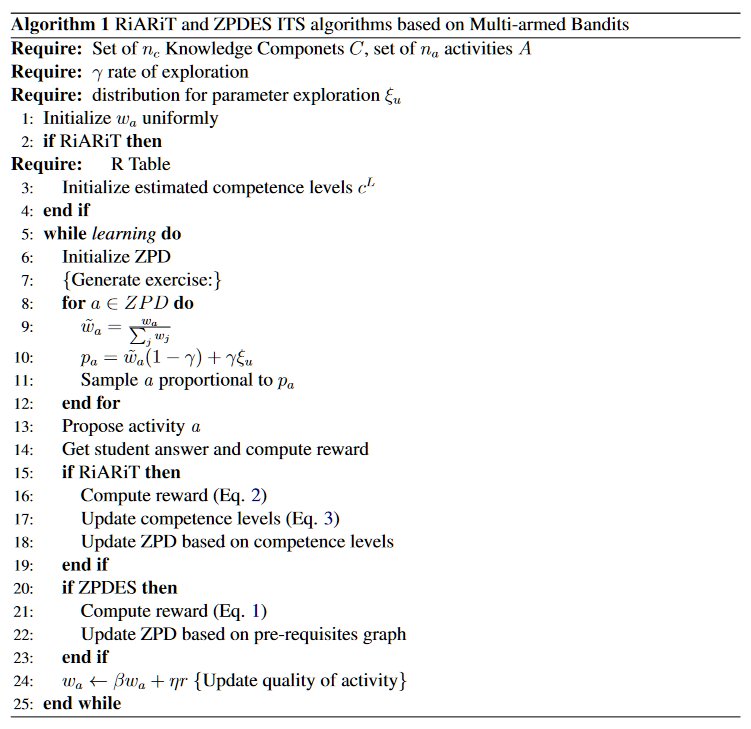
\includegraphics[scale=1]{fig/2Litterature_uncompressed/lopes-alg.png}
\end{center}
\caption{\citet{clement2015multi}'s algorithms}
\label{alg:clement}
\end{figure}

They present two similar algorithms which we reproduce in Figure~\ref{alg:clement}. Each algorithm has two components: the first one computes a \emph{Zone of Proximal Developement} (ZPD, \citet{luckin2001designing}), the second selects one knowledge component in the ZPD. The ZPD aims to exclude the KCs on which the student is either too good, too bad, or the ones on which s/he does not progress.  These algorithms don't use any model nor parametric assumption on the way the student progresses. They compute non-parametric statistics to estimate the current level or the current progress of the student on a KC.

Once the ZPD is set, a bandit algorithm selects a KC. The reward is a difference between the last samples and the before last ones. In the first algorithm (Zone of Proximal Development and Empirical Success - \ZPDES), they use the average of the $\nicefrac{d}{2}$ last samples minus the average $\nicefrac{d}{2}$ before last samples. In the second algorithm (Right Activity at the Right Time - \RiARiT), they use the last sample minus a discounted average of the previous ones. These two statistics measure the recent progress of the students. 

They claim to use a variant of \EXPfour \citep{auer2002nonstochastic}. Like \EXPfour, this algorithm is probabilistic (see Line~11 in Fig.~\ref{alg:clement}). The output probability distribution pulls arm according to weights, which are a weighted sum of rewards. This probability distribution also has a uniform component $\xi_u$, like the vanilla \EXPfour. Notice that this component was later proven to be unnecessary \citep{bubeck2012regret}, even to recover high probability guarantees \citep{neu2015explore}. 

Yet, this bandit algorithm also has major differences with \EXPfour. First, there are no experts recommendations which are a necessary input of \EXPfour. Hence, this algorithm is closer to \EXP. In Subsection~\ref{sec:adv-bandits}, we presented the three ideas beyond \EXP: Follow the regularized leader, a specific regularization, and an unbiased estimation scheme based on importance weight. The specific regularization is responsible for the exponential weights, which are absent from the algorithm of \citet{clement2015multi}. The importance weights of the loss -  the loss is divided by the probability of pulling the arm - are replaced by fixed weights $\beta$ and $\nu$ on the reward (see Line~24). These fixed weights are closer to discounted statistics used in non-stationary bandits (like \DUCB, \citet{kocsis2006discounted, garivier2011upper-confidence-bound}). 

Anyway, the main feature of \EXP is to guarantee $\tcO\pa{\sqrt{KT}}$ regret compared to the sum of the reward for the policies which select always the same arm. In this setup, we believe that the interest of this result is limited for two reasons. First, the policies which selects always the same KCs are not the most interesting policies from the educational point of view. Second, the rewards are weighted differences of past observations. Hence, there is a telescoping effect in the cumulative reward. For some choices of parameters in the reward definition (e.g. $d=2$ for \ZPDES), this telescoping can be total such that the sum of the rewards is simply the last observation minus the first, \ie a $\cO\pa{1}$ quantity. In that case, the $\tcO\pa{\sqrt{KT}}$ guarantee is meaningless. Even for other choices of parameters, the telescoping reduces the cumulative reward range. The more that range is reduced \emph{by construction}, the less interesting is the theoretical guarantee of \EXP.

Hence, we believe that the modifications suggested by \citet{clement2015multi} are indeed more interesting than the classical \EXP. Their algorithm targets a more pragmatic goal: selecting randomly the KCs (to ensure diversity in the tasks) while favoring smoothly the KCs which demonstrate recent progress. They provide empirical evidence of the benefits of their algorithms. In a simulated experiment, they show that their algorithms are more adaptable than an expert sequence to the profile of some simulated students. In an in-class experiment on real students, they show that students who were learning with their algorithms achieve more balanced performance between KCs than a control group that was using the expert sequence. They also demonstrate qualitative differences between the behavior of their algorithm and the expert sequence. 

As noticed by \citet{pikeburke2019phd}, this paper is arguably one of the most advanced works using bandits in ITS. The objective - targeting the topic on which the student progresses - is very appealing. The ZPD design allows some timely exploration by unlocking progressively the most advanced topics. The experiments bring many insightful comparisons between the studied algorithms and the expert sequence. However, this work only partially address the aforementioned shortcomings~\ref{ss:shortcoming-oracle}, \ref{ss:shortcoming-non-stationary}, and~\ref{ss:shortcoming-slow}.

In particular, there are statistical issues with respect to shortcomings~\ref{ss:shortcoming-oracle} and~\ref{ss:shortcoming-non-stationary}. The goal of the paper is to aim at the arm with the current largest increase. It is not clear that this problem fall under the cumulative reward maximisation perspective (see our discussion on the telescoping effect). Even in the algorithm, it is not clear that taking a discounted sum of rewards, which are themselves differences of past observations is a statistically efficient way to measure recent progress. We also notice that these algorithms are quite difficult to tune. They have 4 parameters: $\gamma$, $\nu$, $\beta$ and an other parameter for the reward computation.

The work of \citet{clement2015multi} was further extended by \citet{mu2018combining} to take into account the forgetting of the student and the learning of the ZPD structure. 

We also advertise the works of \citet{rollinson2015predictive, kaser2016stop}, which also try to track the progress of the student. These works do not aim at choosing the knowledge component among several possibilities. Instead, they try to decide when one should stop the work on a given skill. \citet{rollinson2015predictive} suggest stopping when there is a sufficient probability that the prospective learning gain associated with the next question is below a threshold. The prospective learning gains are estimated with a student model. Notice that these models are trained with the data of many other students such as it reflects the "average" student.  The models assume a specific shape of the progression. Hence, different models with the same input sequence can lead to different stopping times, even when they have comparable predictive performance. The issue is that the predictive performance is evaluated on several students, the goal is to predict correctly on average. However, when they are used in instructional policies, these models are required to explain and predict quantitatively the learning of a specific student given a small amount of data. This instructional policy was further extended by \citet{kaser2016stop} to be able to stop when a student's performance diverges from the model (for instance, for wheel-spinning student) and to include more complex student models such as deep belief network. 

\subsection{Target the least known subject}
\label{ss:less-known}
\citet{melesko2019computer} suggest targeting the less known subjects. The idea is that the student has more to learn from their mistakes than from their successes. Hence, they suggest rewarding the failed questions and to not reward the succeeded ones. 

Rewarding the system for finding the failed exercises has some limits. Some skills are harder to get, and it could be useful to start with the simplest one. It can also be the case that there are some prerequisite dependencies between the different skills. From the motivational point of view, recommending too hard questions may disengage the student. 

Yet, consider a student that is learning some geography facts. S/he wants to check if s/he know their lesson. The different topics in the lesson are as hard to learn \emph{a priori}. Yet, the student could have studied a lot the first part of the course and did not spend too much effort on the other parts. The goal of the ITS could be to try to spot the weaker part of the course and teach them with some questions.

Another motivation highlighted by \citet{melesko2019computer} is the pure-exploration setup, where the goal of the ITS is to find the weakest topic to send the information to the teacher. 

\citet{melesko2019computer} suggest using the classical \UCB algorithm. They carry many very small data experiments where the number of topics (arms of the bandits) is of the same order of magnitude as the number of questions (horizon). In this context, they recommend the usage of smaller confidence intervals than classical \UCB. The experiments show improved performance for \UCB compared to the random strategy. 

In their work, \citet{melesko2019computer} neglect the impact of the questions on the knowledge of the student. The goal is not really to teach through questions, but to find the least understood topic. However, it is surprising that they use an exploration-exploitation algorithm instead of a specialized algorithm from the best arm identification literature. 

\citet{teng2018interactive} also target to find the least known questions with multi-armed bandits methods. They suggest an algorithm adapted from the linear bandits' literature where the reward depends linearly on an embedding. The algorithm uses several graphs structuring questions, users, and concepts. These graphs are used to infer a vector representation of the users and questions. They bring theoretical and empirical evidence of the performance of their algorithm. 

\subsection{Target faster learning}
\citet{rafferty2016faster} suggest minimizing the time the student spends to understand a concept. Hence, the cost (negative reward) associated with each pedagogical action is the time the action takes to be completed. They formulate their problem as a Partially Observable Markov Decision Process. Indeed, the student has a knowledge state which is only partially observable by the teacher. The teacher has several actions: some \emph{examples} which teaches the concept to the student, some \emph{quizzes} which retrieves information about the knowledge state of the student, and some \emph{questions with feedback} which do both at the same time.  The goal of the learner is to track the state of the student (which encodes what the student does not know) with questions to show some relevant examples. 

They test this framework with several student models and several learning scenarios. The algorithm shows significant time reduction compared to random policies. Some student models are better than others. In particular, modeling long-term memory improves performance compared to models that react only to the last seen example.

